\documentclass[cnatzke_thesis_proposal.tex]{subfiles}
\begin{document}

\chapter{Experimental Setup}

%------------------------------------------
\subsection{Data Collection}
%------------------------------------------
Measuring two-photon decay is very challenging due to its small branching ratio and continuum of energy meaning the choice of source is very important.
Historically two-photon decay has been measured using a dedicated decay station and radioactive ion beam (RIB)~\cite{kramp_nuclear_1987}.
The first excited and ground state in $^{90}$Zr are $0^+$ states, with a two-photon transition already observed~\cite{schirmer_double_1984}, and the first excited state is accessible by a $^{90}$Sr source.
$^{90}$Sr sources are typically used as beta particle detector calibration sources since it primarily decays to the ground state of $^{90}$Y then to the ground state of $^{90}$Zr, but there is a 0.012 percent branching ratio from $^{90}$Y to the first excited stat of $^{90}$Zr.
Figure~\ref{fig:decay_scheme_with_twophoton} shows the full decay scheme for a $^{90}$Sr source.

\begin{figure}[H]
  \centering
  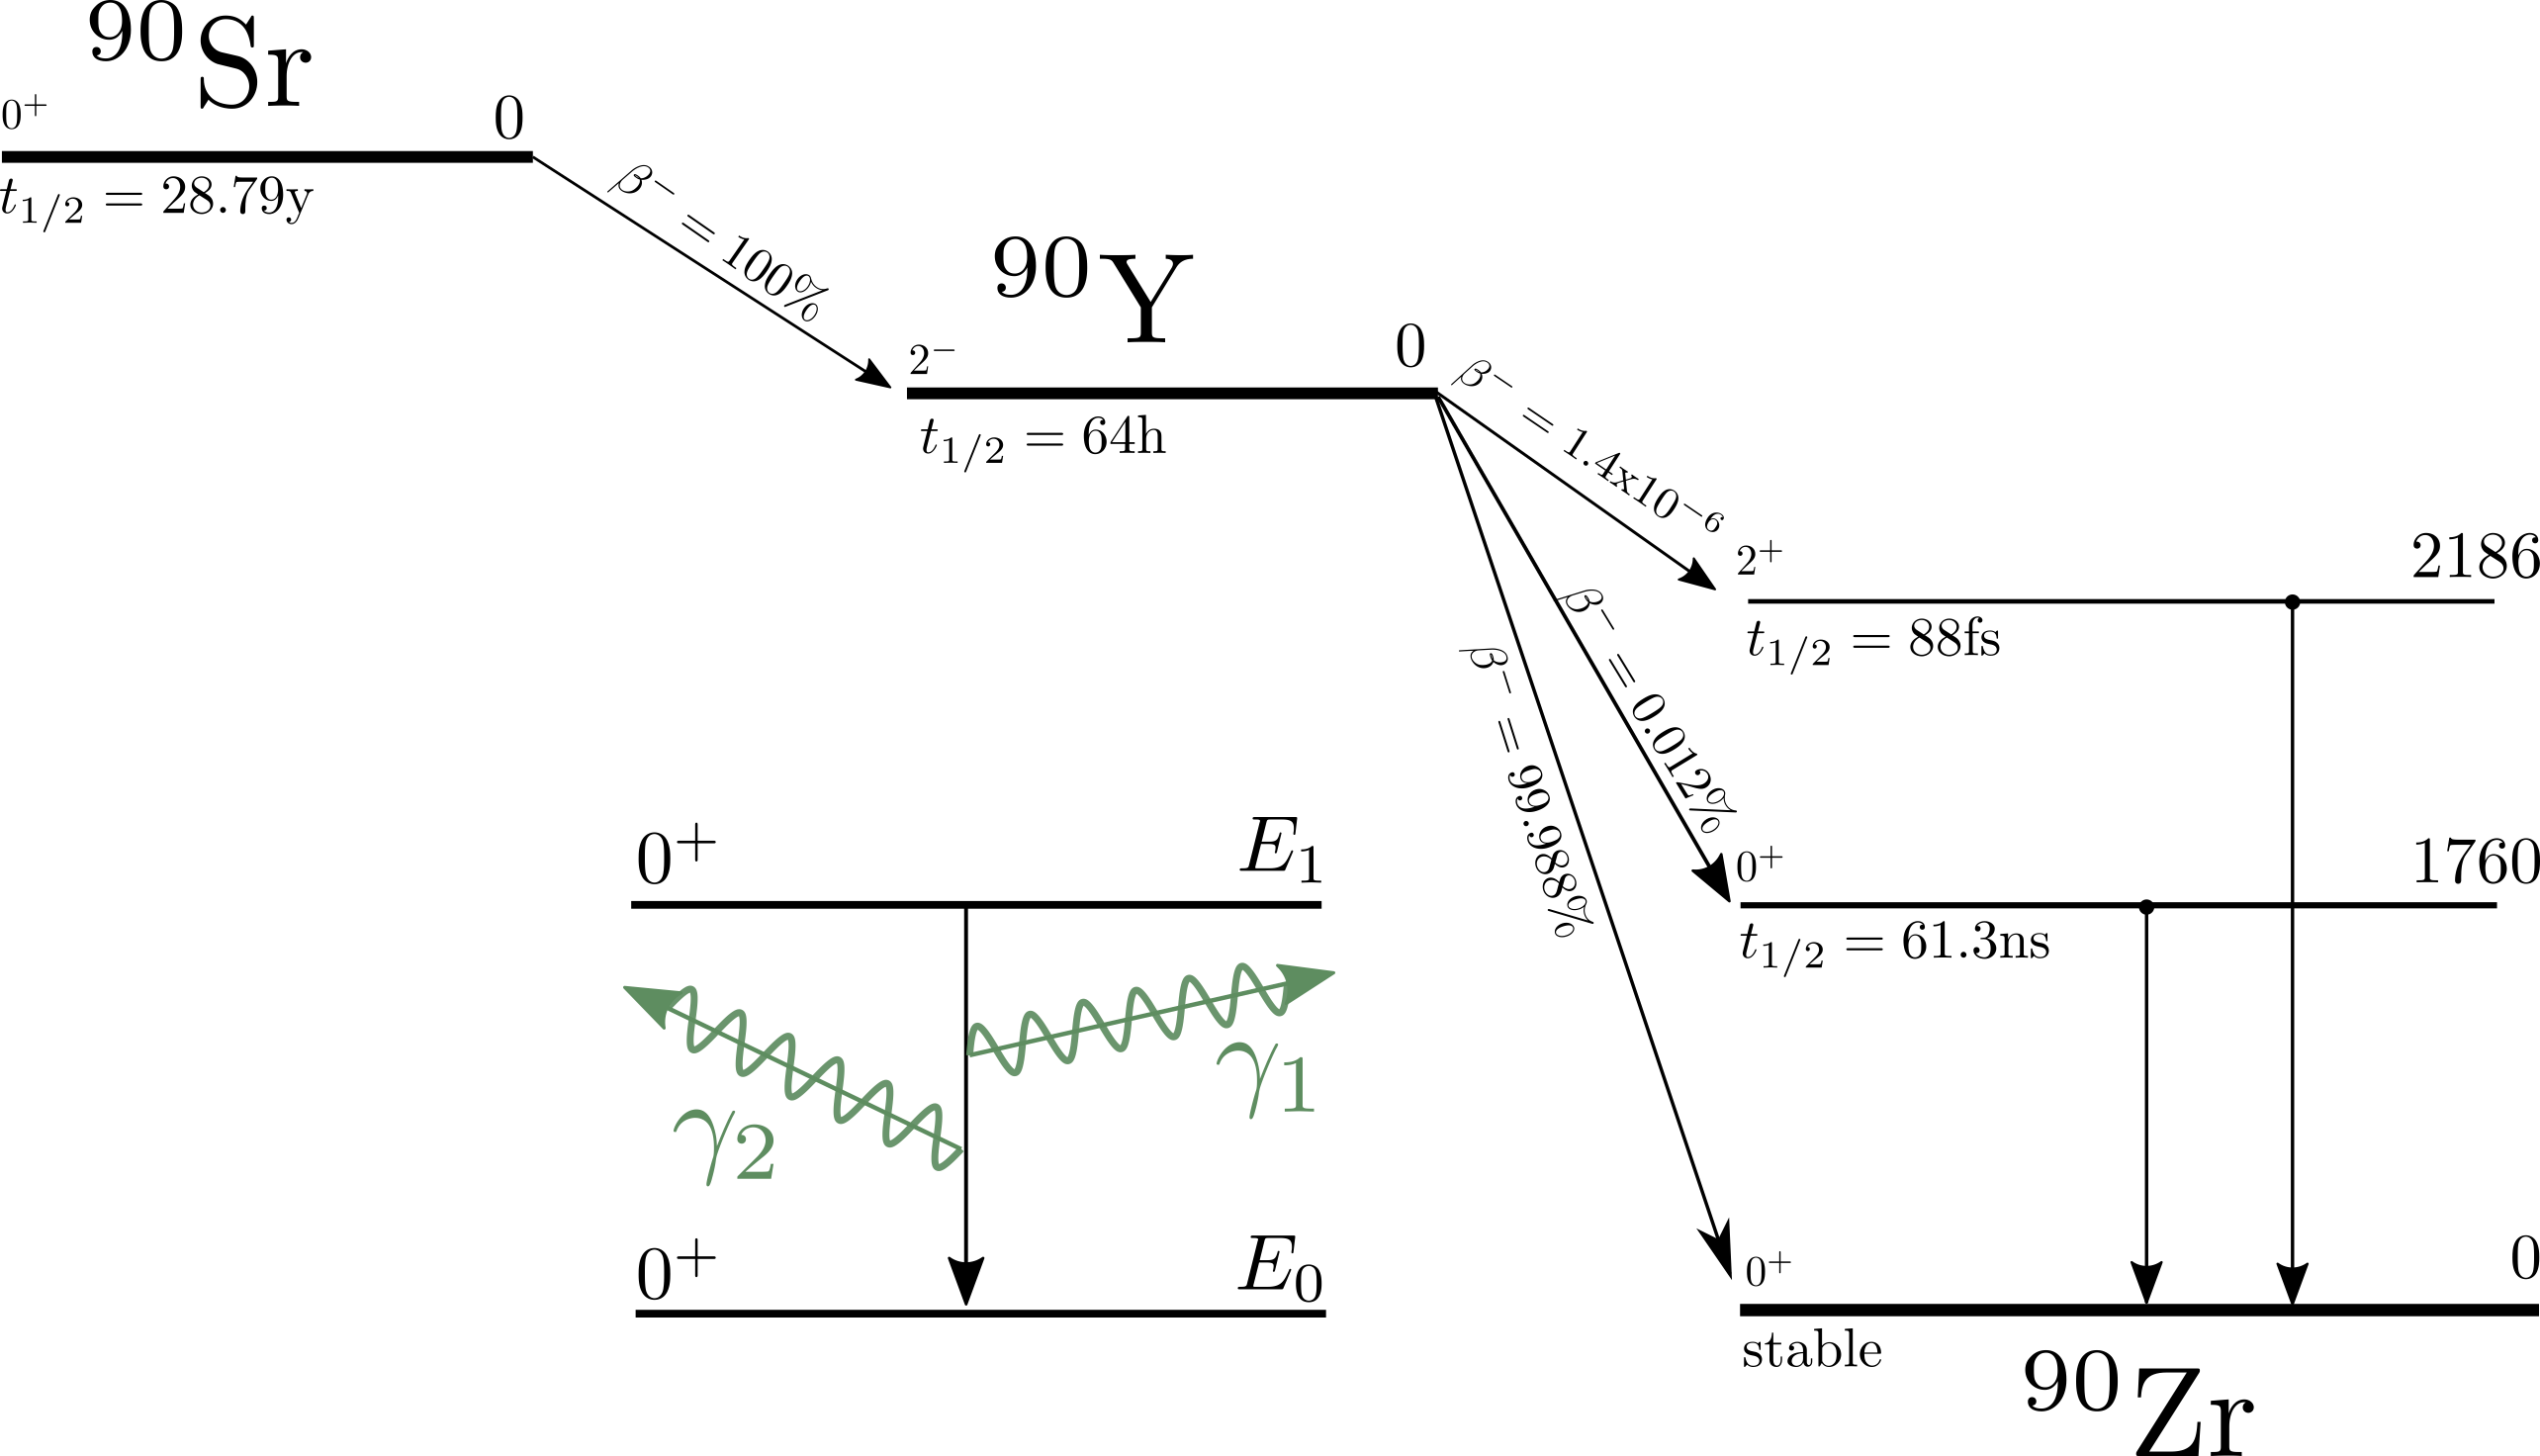
\includegraphics[width=0.95\textwidth]{decay_scheme_with_twophoton.png}
  \caption{Decay scheme of a $^{90}$Sr source with the insert schematically detailing non-competitive two-photon decay.}
  \label{fig:decay_scheme_with_twophoton}
\end{figure}

Since the $E0$ transition of interest in $^{90}$Zr can be accessed without need of a RIB collection time is no longer an issue.
The source can be placed in GRIFFIN and data can be collected for as long as the array is available.

%------------------------------------------
\end{document}
